\newpage
\section[Фигуры 3, 4]{Фигуры 3, 4}

Для построения \textit{фигуры 3}: строим две взаимно перпендикулярные прямые, 
применяем инструмент \textit{\textbf{Interpolate}},
дублируем полученное множество кривых, осуществляем поворот.

Для построения \textit{фигуры 4} перемещаем одну из прямых <<вниз>>, далее
порядок построения аналогичен \textit{фигуре 3}.
\vspace{12pt}

Ниже приведены этапы построения фигур 3 и 4:
\begin{figure}[H]
    \begin{minipage}[h]{1\linewidth}
        \center{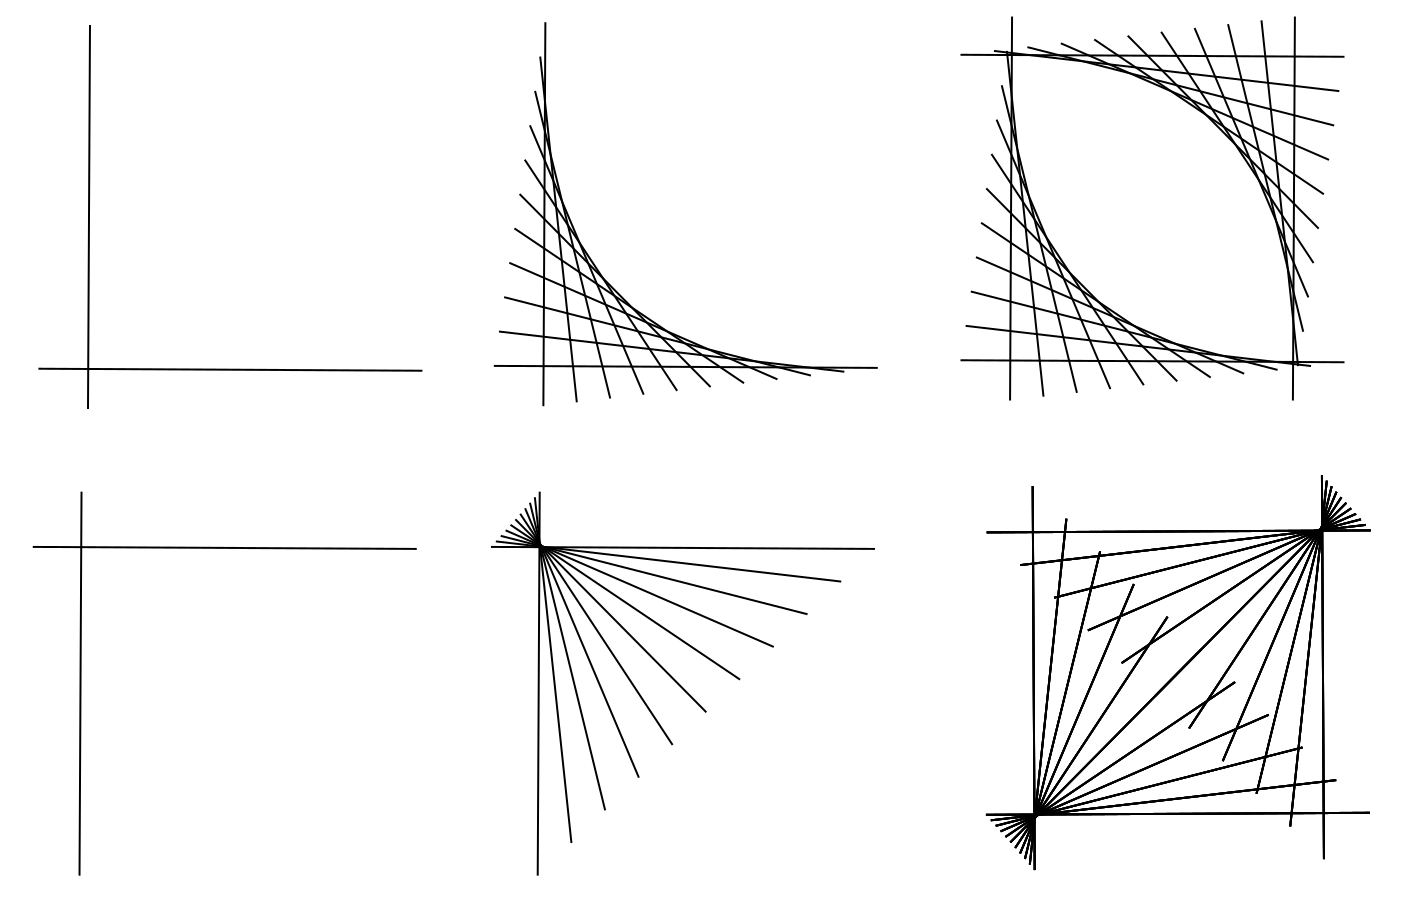
\includegraphics[width=1\linewidth]{3_pic.png}}
    \end{minipage}
\end{figure}

Таким образом убеждаемся в зависимости результата построения групп перетекания 
от направления построения кривых (прямых).
